\documentclass[10pt,final]{scrreprt}
\usepackage[T1]{fontenc}
\usepackage[utf8]{inputenc}
\usepackage{graphicx}
\usepackage{tabularx}
\usepackage{psfrag}
\usepackage[monochrome]{epsfig}
\usepackage{amsfonts,amssymb,amsmath}
\usepackage{url} 
\usepackage{fullpage} 
\usepackage{appendix}
\usepackage{textcomp}
\usepackage{listings} 
\usepackage{color} 
%\usepackage[ps2pdf,colorlinks=true]{hyperref}%colorlinks bewirkt rote links, gut fuer debug
\usepackage{hyperref}
\usepackage{tikz}
\usepackage{verbatim}
\usepackage{tikz}
\usepackage{times}



\newcommand{\unityvrrepos}{\url{ssh://ai.informatik.tu-chemnitz.de//work/mercurial/vrNeuroStable}} 

\usetikzlibrary{arrows,shapes,positioning,shadows,trees}
\newcommand*\circled[1]{\tikz[baseline=(char.base)]{
            \node[shape=circle,draw,inner sep=2pt] (char) {#1};}}

\definecolor{grey}{rgb}{0.95,0.95,0.95} 

\linespread{1.1} %Zeilenabstand

%absatzeinzuge
\setlength{\parindent}{0mm} %bei neuem Absatz nicht einruecken
\setlength{\parskip}{0.4em} % 0.4 Zeile bei neuem Absatz
\setcounter{tocdepth}{2}%tiefe des inhaltsverzeichnisses


\tikzset{
  basic/.style  = {draw, text width=2cm, drop shadow, font=\sffamily, rectangle},
  root/.style   = {basic, rounded corners=2pt, thin, align=center,
                   fill=green!30},
  level 2/.style = {basic, rounded corners=6pt, thin,align=center, fill=green!60,
                   text width=8em},
  level 3/.style = {basic, thin, align=left, fill=pink!60, text width=6.5em,align=center},
  level 4/.style = {basic, thin, align=left, fill=yellow!60, text width=6.5em,align=center,grow=down},
  level 5/.style = {basic, thin, align=left, fill=white!60, text width=6.5em,align=center,grow=down}
}


\begin{document}

\title{UnityVR User Manual}
%\subtitle{Revision 2.3, SVN-Revision R372}
\author{Michael Schreier}
%\date{10.08.2013}
\maketitle

\tableofcontents
\lstset{numbers=none, tabsize=2, frame=single, breaklines=true, basicstyle=\small\ttfamily,
   numberstyle=\tiny\ttfamily, framexleftmargin=3mm, backgroundcolor=\color{grey}, xleftmargin=2mm}

%CHAPTER%%%%%%%%%%%%%%%%%%%%%%%%%%%%%%%%%%%%%%%%%%%%%%%%%%%%%%%%%%%%%%
\chapter*{Outline}
The neuronal agents and their virtual environment (VR) are simulated on a distributed and specialized device. The agents have all main abilities of a human, they are capable to execute simple actions like moving or jumping, to move their eyes and their heads and to show emotional facial expressions. Agents learn their behavior autonomously based on their actions and the resulting sensory consequences in the environment. For this purpose, the VR-engine contains a rudimentary action- and physic-engine. Small movements (like stretching the arm) are animated by the VR-engine, while the neuronal model rather controls high-level action choices like grasping a certain object.

Unity3D is used as VR-Engine for UnityVR. Unity3D was chosen as it is an easy to use cross-platform game or VR engine. This document is the user manual. If you look for further development informations refer the Development Manual (\emph{[Repository directory]/unityVR/doc/VR-doc}).  

\begin{itemize}
\item Chapter 1 starts with a short instruction of Unity3D and its IDE. It also explains the importing of the project UnityVR. It will not cover details or features of Unity3D. If  you want to learn more about Unity3D, please visit the Unity3D homepage (\url{http://www.unity3d.com}).

\item Chapter 2 shows the UnityVR workflow by example and describes all essential parts of it. We will create a simple environment and the connection to the neuronal network simulator ANNarchy. All scipts/classes of UnityVR are written in the C\# language whereby the ANNarchy client is written in C++. Because of that, some basic knowlege of both languages is required. 

\item Chapter 3 gives a more detail overview of UnityVR. For a full overview refer to the development documentation (doc/VR-doc/html/index.html).

\item Chapter 4 covers further infomation and tips about useful features of Unity3D and the design workflow.
\end{itemize}
%CHAPTER%%%%%%%%%%%%%%%%%%%%%%%%%%%%%%%%%%%%%%%%%%%%%%%%%%%%%%%%%%%%%%
\chapter{Basics of Unity}
\label{basicsofunity}



Unity3D is a game engine with a build-in IDE. It is suited for easy developing of 3D games. This chapter will give a short overview over  the IDE and its features. For further details refer the Unity3D documentation ({\url{http://unity3d.com/learn/documentation}}).

%SECTION%%%%%%%%%%%%%%%%%%%%%%%%%%%%%%%%%%%%%%%%%%%%%%%%%%%%%%%%%%%%
\section{Installation}
\label{Installationofunity}

You can obtain Unity3D from 
\begin{itemize}
\item  Official homepage (\url{http://unity3d.com/unity/download})
\item For older Unity3D versions go to \url{http://unity3d.com/unity/download/archive}
\end{itemize}

You could get a 30 day trail for free, but some parts of UnityVR (RenderTextures) require a Unity3D professional license.  It is advised to use Unity-Version 4.2.0, provided under unityVR\_xxx/install/UnitySetup-4.2.0.exe

%SECTION%%%%%%%%%%%%%%%%%%%%%%%%%%%%%%%%%%%%%%%%%%%%%%%%%%%%%%%%%%%%
\section{Elements of the IDE}
\label{elementsofIDE}

\begin{figure}[h]
\begin{center}
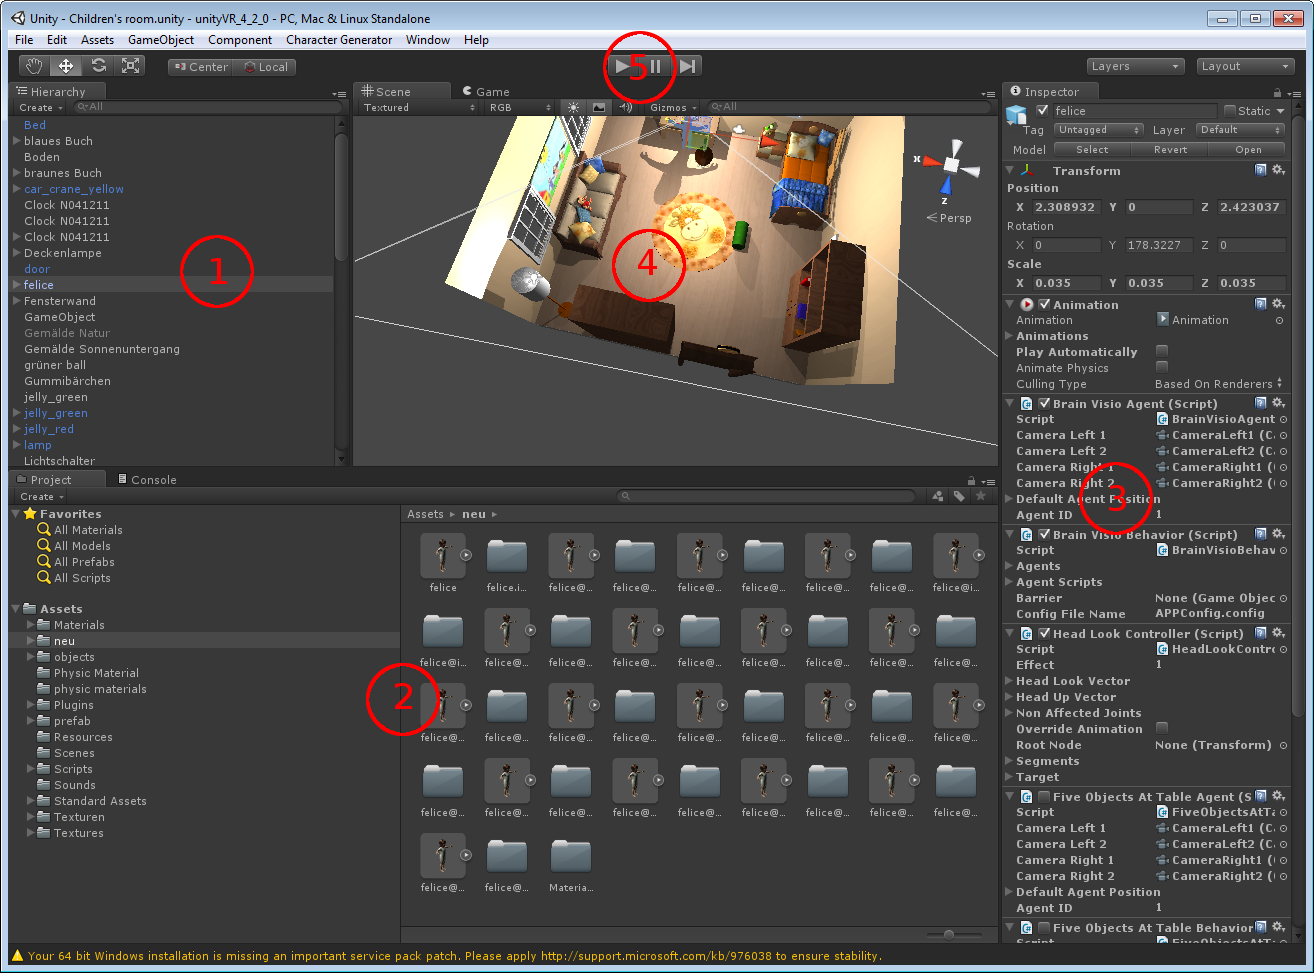
\includegraphics[width=0.95\textwidth]{images/unitywindow2.png}
\end{center}
\caption{Unity3D IDE (Version 4.2.0f)}
\label{unitywindow}
\end{figure}

This section will give a short overview about Unity3D. Fig. \ref{unitywindow} shows the IDE of Unity3D 4.2.0f.

\begin{description}
\item[\circled{1}] \textbf{Scene Graph} \\ Tree View of all currently present objects in the active scene.
\item[\circled{2}] \textbf{Project View} \\ Shows the directory structure and all files that are contained in the \emph{Assets} folder.
\item[\circled{3}] \textbf{Object Inspector} \\ Shows details and attached components/scripts of the currently selected object.
\item[\circled{4}] \textbf{Scene} \\ This is the development view of the actual scene. Here you can add objects to the scene or modify objects.
\item[\circled{5}] \textbf{Start/Pause/Stop} \\ Starts/pauses or stops the game engine for playback in the editor.
\end{description}


%SECTION%%%%%%%%%%%%%%%%%%%%%%%%%%%%%%%%%%%%%%%%%%%%%%%%%%%%%%%%%%%%
\newpage
\section{First Time Importing the Project}
\label{importingproject}

\begin{enumerate}
\item Checkout the latest UnityVR Release from via HG from \unityvrrepos.\\The recommended HG tool for Windows is TortoiseHG (\url{http://tortoisehg.bitbucket.org}).
\item Click on \emph{"Open Project"} in the \emph{"File"} menu. The Project Wizard will popup (Fig. \ref{imgprojectwizard}).
\item Now click on the \emph{"Open other..."} button and choose the directory which contains the project. This will start a new  instance of Unity3D and the  import status window appears (Fig. \ref{imgimportprogress}). 
This process can take up to 30 minutes depending on the computer and project size.
\item[Note:] Make sure to run Unity with a proper GPU.
\end{enumerate}


\begin{figure}[h]
\begin{center}
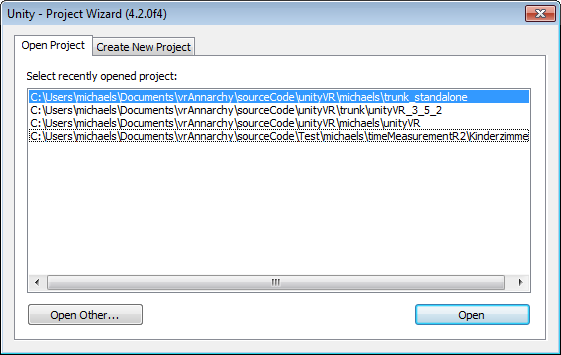
\includegraphics{images/projectwizard.png}
\end{center}
\caption{The Project Wizard shows recently opened projects. The \emph{"Open other..."} button lets you open another already existing Project.}
\label{imgprojectwizard}
\end{figure}


\begin{figure}[h]
\begin{center}
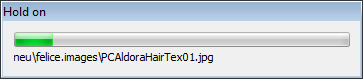
\includegraphics{images/importprogress.png}
\end{center}
\caption{This windows shows the actual import progress. Depending on the PC and the Project, it can take a long time.}
\label{imgimportprogress}
\end{figure}

\newpage


\chapter{Creating New Scene by Example}

This chapter describes the creation of a minimal scene in Unity3D step by step. We begin with an empty scene where we are going to create a simple environment with an agent with all essential scripts and the connection with ANNarchy.

%\section{Download UnityVR}

 %Download the Unity-Project via subversion from : \url{https://ai.informatik.tu-chemnitz.de/repos/vrAnnarchy/sourceCode/releases/unityVR_xxxxxx/} or from the AI-software repository (UnityVR Revision xxxxxx).

%Currently (10.8.2013), no release is available, please use the latest trunk version: \url{https://ai.informatik.tu-chemnitz.de/repos/vrAnnarchy/sourceCode/unityVR/trunk/unityVR_4_2_0}. The resulting folder is called in this text now 'unityVR\_xxx'.
%The unity-project file could then found under\\\textsf{unityVR\_20120523/unityVR/Assets/Scenes/Children's room.unity}

%The main-config file is the unityVR\_xxx/APPConfig.config (should be copied from install/) and the documentation can be found under unityVR\_xxx/doc. 


\section{UnityVR Design / Code}


These following steps describe the necessary procedures in Unity3D to create a new environment with the agent Felice and are done inside the UnityVR project. Make sure you import of UnityVR into Unity3D properly as descripted in \ref{importingproject}.

\subsection{Creating the Environment}
\begin{enumerate}
\item Click the \emph{File} menu and choose \emph{New Scene}.
\item Click the \emph{File} menu and choose \emph{Save Scene}. Save it into the \emph{Assets/Scene} Folder and choose a descriptive filename.
\end{enumerate}

 Now we have empty scene (Fig. \ref{imgemptyscene}). In the following step we want to create a floor, a table, lights and the agent.


\begin{figure}[p]
\begin{center}
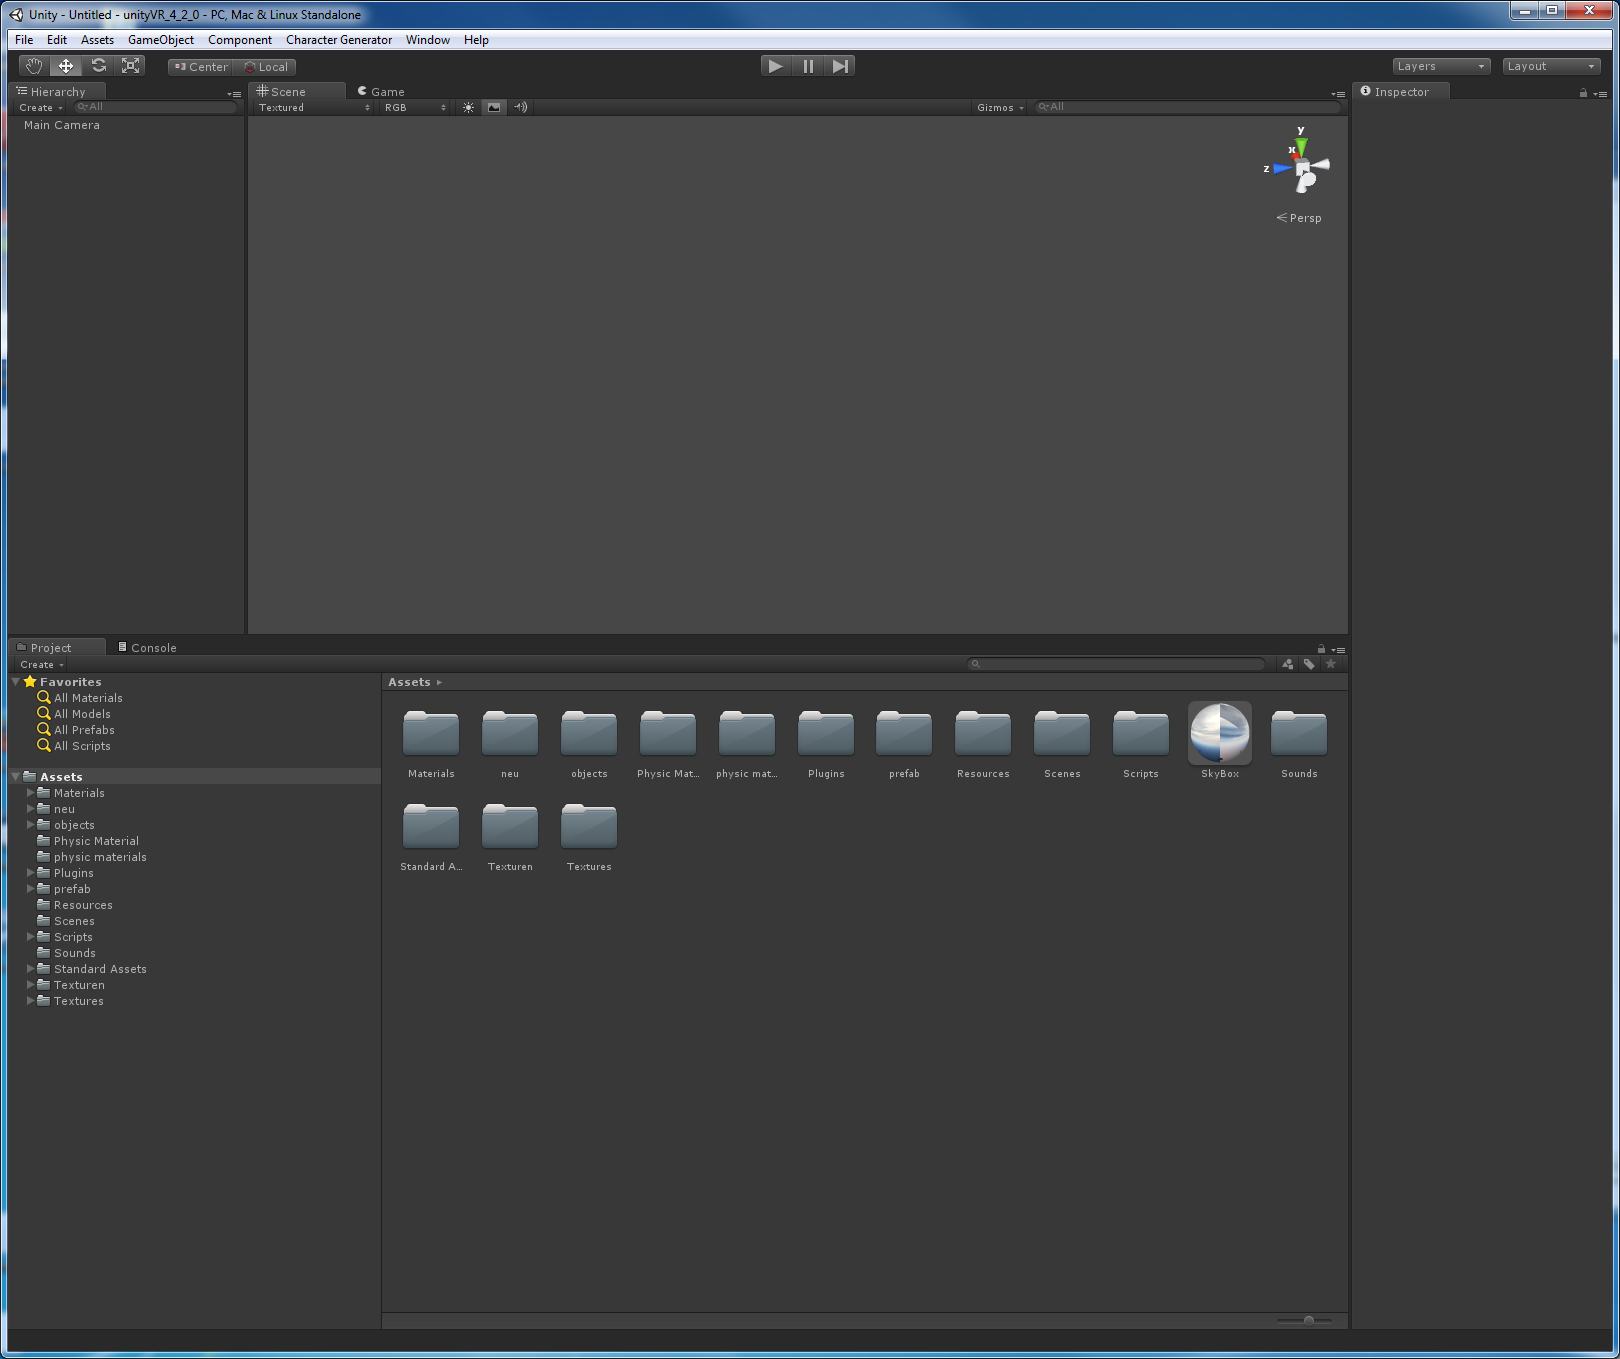
\includegraphics[width=0.70\textwidth]{images/emptyscene.png}
\end{center}
\caption{ View of a new created scene}
\label{imgemptyscene}
\end{figure}

\begin{figure}[p]
\begin{center}
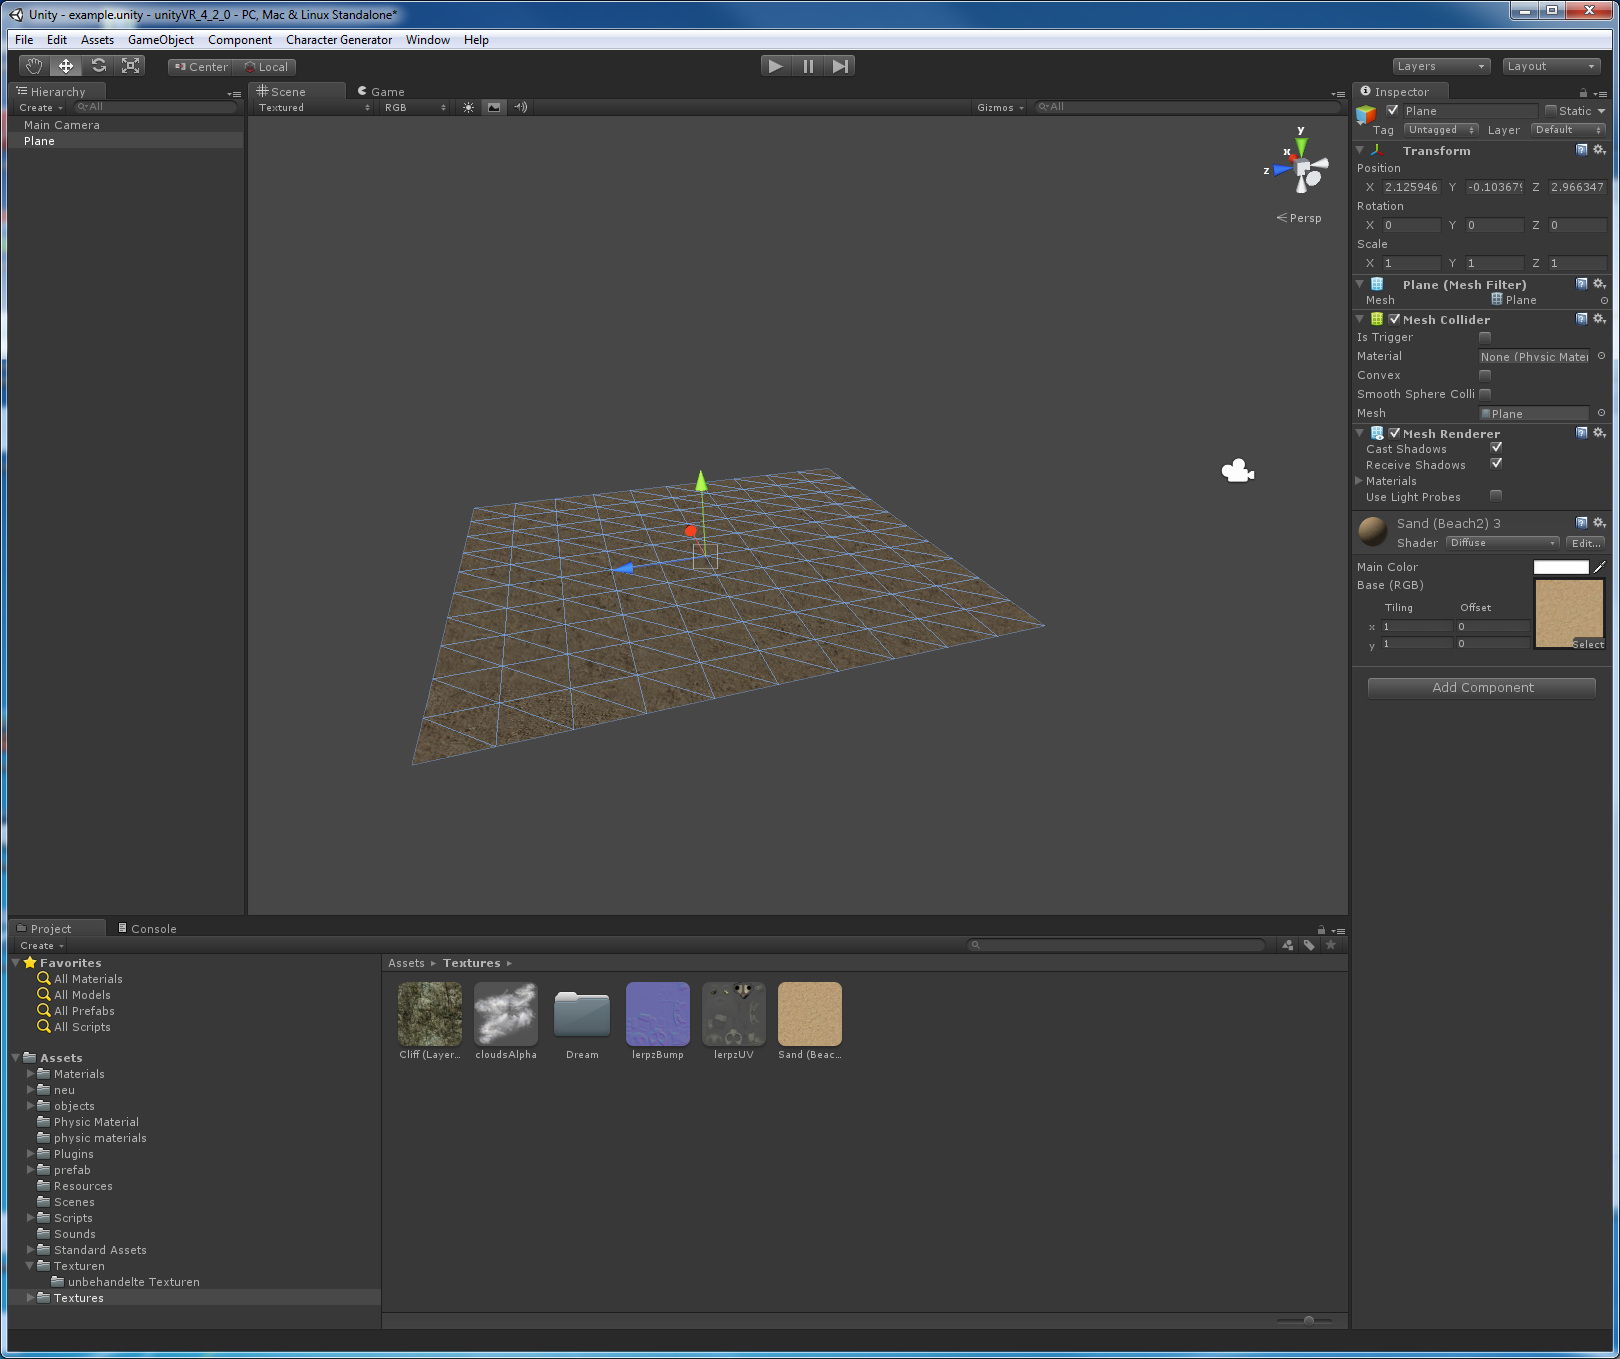
\includegraphics[width=0.70\textwidth]{images/scenewithfloor.png}
\end{center}
\caption{Editor View with the instantiated floor plane}
\label{imgscenewithfloor}
\end{figure}

\begin{enumerate}
\setcounter{enumi}{2}
\item We need a floor, on which the agent can walk. Click the \emph{GameObject} menu,  sub menu \emph{Create Other} and choose \emph{Plane}. A \emph{plane} has an already attached mesh collider, which is needed, so that the agent does not fall through the floor.
\item Go to the \emph{Texture} folder in the Project View and attach a texture on the new created plane via drag and drop (Fig. \ref{imgscenewithfloor}).
\item Go into \emph{objects/common} folder, select the \emph{table} object and drag it into the scene. We have to scale the table down, to make it smaller. The easiest way to do that is to ajust the scale values in the Object Inspector. I chose the value 0.05 for \emph{X}, \emph{Y} and \emph{Z} (Fig. \ref{imgscenetable}). Optionally, you could add a \emph{BoxCollider} and a \emph{Rigidbody} to the table to enable collision detection and physics respectively.
\item We create a light source.  Click the \emph{GameObject} menu,  sub menu \emph{Create Other} and choose \emph{Point Light}. Drag it to a spot in the scene and change its values in the Object Inspector as you wish.
\item Adjust the values of the \emph{Main Camera}  so that the environment is visible in the Camera View.
\end{enumerate}

\begin{figure}[h]
\begin{center}
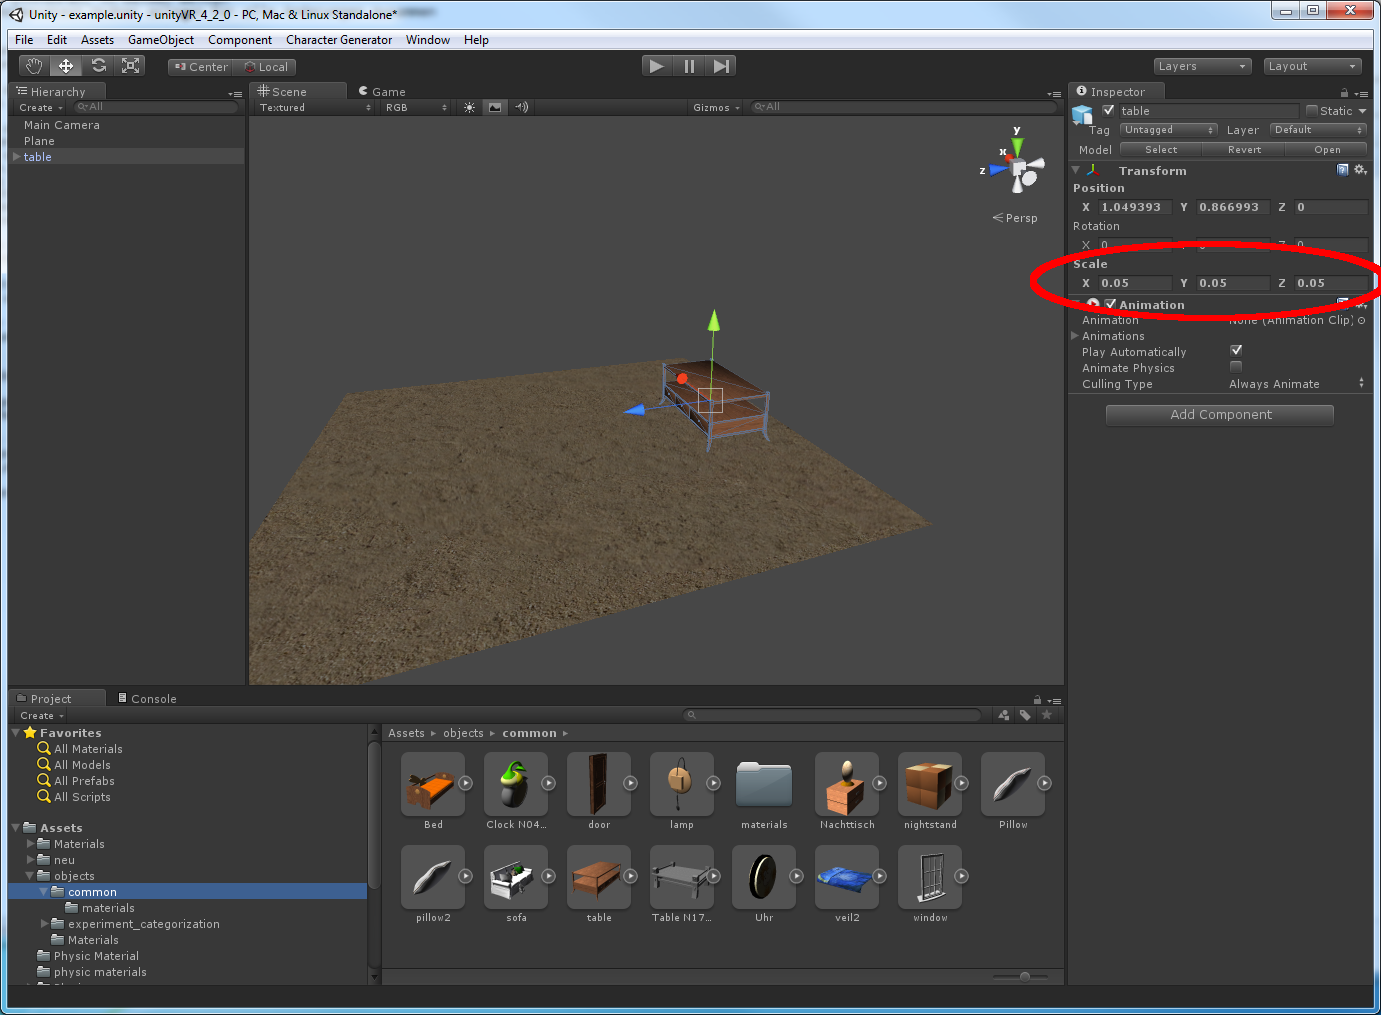
\includegraphics[width=0.80\textwidth]{images/scenetable.png}
\end{center}
\caption{Scene with table. The red ellipse shows the scale options in the Object Inspector.}
\label{imgscenetable}
\end{figure}

Our VR environment is finished. Now we start with the controlling scripts.

\begin{enumerate}
\setcounter{enumi}{7}
\item Create an empty object ( \emph{GameObject->Create Empty} ). Name it \emph{MasterObject}.
\end{enumerate}


Now we attach a derived \emph{BehaviorScript} to the \emph{MasterObject} created in the last step.
The \emph{BehaviorScript} is the main control script in UnityVR. It is responsible for controlling the environment and initialization of the agents. The behavior to messages from the ANNarchy client can be changed by overriding functions in a derived class of \emph{BehaviorScript}. Even if you do not want to change the behavior, it is not intended to use the base class \emph{BehaviorScript} directly. As a convention, you should  always create a derived class from \emph{BehaviorScript}. Also the \emph{BehaviorScript.AgentInitalization} function needs information about the type of the \emph{AgentScript} which we will create later. 

\begin{enumerate}
\setcounter{enumi}{8}
\item We create the new class \emph{ExampleBehaviorScript}. In the example of a \emph{BehaviorScript} below we will override the \emph{AgentInitalization} and \emph{ProcessTrialReset} function. 
\end{enumerate}

%\hspace*{0.2\textwidth}
%\begin{minipage}{0.8\textwidth}
\begin{lstlisting}
using System;
using System.Collections;
using SimpleNetwork;
using UnityEngine;
public class ExampleBehaviorScript : BehaviourScript
{
    protected override void AgentInitalization()
    {
        getAllAgentObjects<ExampleAgentScript>();
        getAndInitAllAgentScripts<ExampleAgentScript>();
    }

    protected override void ProcessTrialReset()
    {
       Debug.Log("Trial Reset received");
       base.ProcessTrialReset();
    }
}


\end{lstlisting}
%\end{minipage}

\begin{enumerate}
\setcounter{enumi}{9}
\item Attach the \emph{ExampleBehaviorScript} to the \emph{MasterObject}.
\end{enumerate}

\subsection{Creating the Agent}
\label{createagent}



\begin{enumerate}
%\setcounter{enumi}{2}
\item Now drag the agent \emph{Felice}  (file ./\emph{animation}/\emph{Felice\_grasp.fbx}) into the scene. Change the scale values appropriate e.g. 0.02 for \emph{X}, \emph{Y} and \emph{Z}.
\item Change the tag of Felice to "agent". So the initializing function of \emph{ExampleBehaviorScript} is able to find Felice.
\item Disable \emph{Play Automatically} in the animation settings of Felice.
\item The most importent script, that must be attached, is an \emph{AgentScript}. It is the main control script of an agent instance. \emph{AgentScript} controls the responses of the agent to messages from the client. Like the \emph{BehaviorScript}, the \emph{AgentScript} is intended to be derived. The following code shows the \emph{ExampleAgentScript} which must be attached to the agent.
\end{enumerate}

\begin{lstlisting}
using System;
using System.Collections;
using SimpleNetwork;
using UnityEngine;

public class ExampleAgentScript : AgentScript
{
	protected override void ProcessMsgAgentGraspID( MsgAgentGraspID msg )	
	{
        		Debug.Log("AgentGraspID received");
	}

}
\end{lstlisting}


\begin{enumerate}
\setcounter{enumi}{3}
\item There are serveral other components from Unity3D and the \emph{Assets/Scripts} folder that must be attached directly % (if not described differently)
to our agent \emph{Felice} to get it working:
\begin{itemize}
\item \emph{Component -> Physics -> Character Controller}\footnote{\url{http://docs.unity3d.com/Documentation/Components/class-CharacterController.html}}
\begin{itemize}
\item Set the values for \emph{Center} to [0, 51, 0], \emph{Radius} to 14 and \emph{Height} to 100. The agent will be inside the collider of the \emph{Character Controller}.
\end{itemize}
\item \emph{Controller Collider} script (responsible for collision detection)
\item \emph{HeadLookController} script (head rotation of the agent)
\item Add 4 cameras to the agent object, two for each eye.\footnote{One camera (no. 1) renders the Eye View to be displayed in the running VR. The other one (no. 2) renders the Eye View for the connected client.}
\begin{itemize}
\item Name them \emph{CameraLeft1}, \emph{CameraLeft2}, \emph{CameraRight1} and \emph{CameraRight2}.
\item Deactivate the \emph{Audio Listener} in the editor for all four cameras.
\item Adjust the postition of the cameras so that they match with the eyes of the agent. 
\begin{itemize}
\item \emph{CameraLeft1} and  \emph{CameraLeft2} for the left eye at position [-4.2, 84.5, 8]
\item \emph{CameraRight1} and  \emph{CameraRight2} for the right eye at position [1.5, 84.5, 8]
\end{itemize}
\end{itemize}
\end{itemize}
\end{enumerate}



\newpage
\subsection{APPConfig.config}

The config file of UnityVR is \emph{APPConfig.config}. It is located in the root directory of UnityVR.  For a description of all parameters look at \ref{appconfig}. For this example your \emph{APPConfig.config} should look like the following listing.



\begin{lstlisting}
<?xml version="1.0" encoding="UTF-8"?>
<cConfiguration xmlns:xsi="http://www.w3.org/2001/XMLSchema-instance" xmlns:xsd="http://www.w3.org/2001/XMLSchema">
  <LocalPort>1337</LocalPort>
  <SyncMode>false</SyncMode>
  <SimulationTimePerFrame>0.1</SimulationTimePerFrame>
  <ImageResolutionWidth>1024</ImageResolutionWidth>
  <SendGridPosition>true</SendGridPosition>
  <MovementSpeed>3</MovementSpeed>
  <CameraDisplayWidth>512</CameraDisplayWidth>
  <FovHorizontal>120</FovHorizontal>
  <FovVertical>90</FovVertical>
</cConfiguration>
\end{lstlisting}


\section{ANNarchy/C++ Client}


The environment and the agent have seperate TCP sockets to communicate with the client. The IP address  is the IP of the computer where Unity3D is executed. The ports are chosen by the user in the \emph{APPconfig.config} file with the \emph{LocalPort} property. The environment has the port \emph{LocalPort} whereby the agent has the port number \emph{LocalPort+agentID+1}, whereby \emph{agentID} is a property of \emph{AgentScript}.

The following code shows an example \emph{main.cpp} for the client. You find this file as \emph{example-main.cpp} in the same folder as this document.\footnote{doc/user-doc/example-main.cpp} You need to change the IP address in line 16 to match with to PC where UnityVR is running. To compile and run it follow the steps in \ref{ConnectionwithANNarchy}.


\lstinputlisting{example-main.cpp}

See also \emph{agentBrain/networkInterfaceCPP/Tests/src/main.cpp} for more examples.

\begin{comment}
\section{Config File --- APPConfig.config }
\label{appconfig}

The \textsf{APPConfig.config} is located in the project folder. 

\begin{lstlisting}
<?xml version="1.0" encoding="Windows-1252"?>
<cConfiguration xmlns:xsi="http://www.w3.org/2001/XMLSchema-instance" xmlns:xsd="http://www.w3.org/2001/XMLSchema">
  <LocalPort>1337</LocalPort>
  <SyncMode>false</SyncMode>
  <SimulationTimePerFrame>0.1</SimulationTimePerFrame>
  <ImageResolutionWidth>256</ImageResolutionWidth>
  <ImageResolutionHight>256</ImageResolutionHight>
  <SendGridPosition>true</SendGridPosition>
  <MovementSpeed>10</MovementSpeed>
  <CameraDisplayRes>256</CameraDisplayRes>
</cConfiguration>
\end{lstlisting}

\begin{lstlisting}
<?xml version="1.0" encoding="UTF-8"?>
<cConfiguration xmlns:xsi="http://www.w3.org/2001/XMLSchema-instance" xmlns:xsd="http://www.w3.org/2001/XMLSchema">
  <LocalPort>1337</LocalPort>
  <SyncMode>false</SyncMode>
  <SimulationTimePerFrame>0.1</SimulationTimePerFrame>
  <ImageResolutionWidth>256</ImageResolutionWidth>
  <ImageResolutionHight>256</ImageResolutionHight>
  <SendGridPosition>true</SendGridPosition>
  <MovementSpeed>4</MovementSpeed>
  <CameraDisplayWidth>400</CameraDisplayWidth>
  <FovHorizontal>120</FovHorizontal>
  <FovVertical>90</FovVertical>
</cConfiguration>
\end{lstlisting}
\end{comment}


%CHAPTER%%%%%%%%%%%%%%%%%%%%%%%%%%%%%%%%%%%%%%%%%%%%%%%%%%%%%%%%%%%%
\chapter{UnityVR User Reference}
\label{basicsofunityvr}


%SECTION%%%%%%%%%%%%%%%%%%%%%%%%%%%%%%%%%%%%%%%%%%%%%%%%%%%%%%%%%%%%
\section{Download UnityVR}

 Download the Unity-Project via Mercurial from : \unityvrrepos  or from the AI-software repository (UnityVR Revision xxxxxx).

You can donwload Unity from thier website (\url{https://unity3d.com/get-unity}). We highly recommend the use of the same Unity version as the existing project was created with - currently 4.2.0. Unity archives: \url{https://unity3d.com/get-unity/download/archive} 

The main-config file is the unityVR\_xxx/APPConfig.config (should be copied from install/) and the documentation can be found under unityVR\_xxx/doc. 

%SECTION%%%%%%%%%%%%%%%%%%%%%%%%%%%%%%%%%%%%%%%%%%%%%%%%%%%%%%%%%%%%
\section{Project Folder Structure}
\begin{comment}
\begin{center}
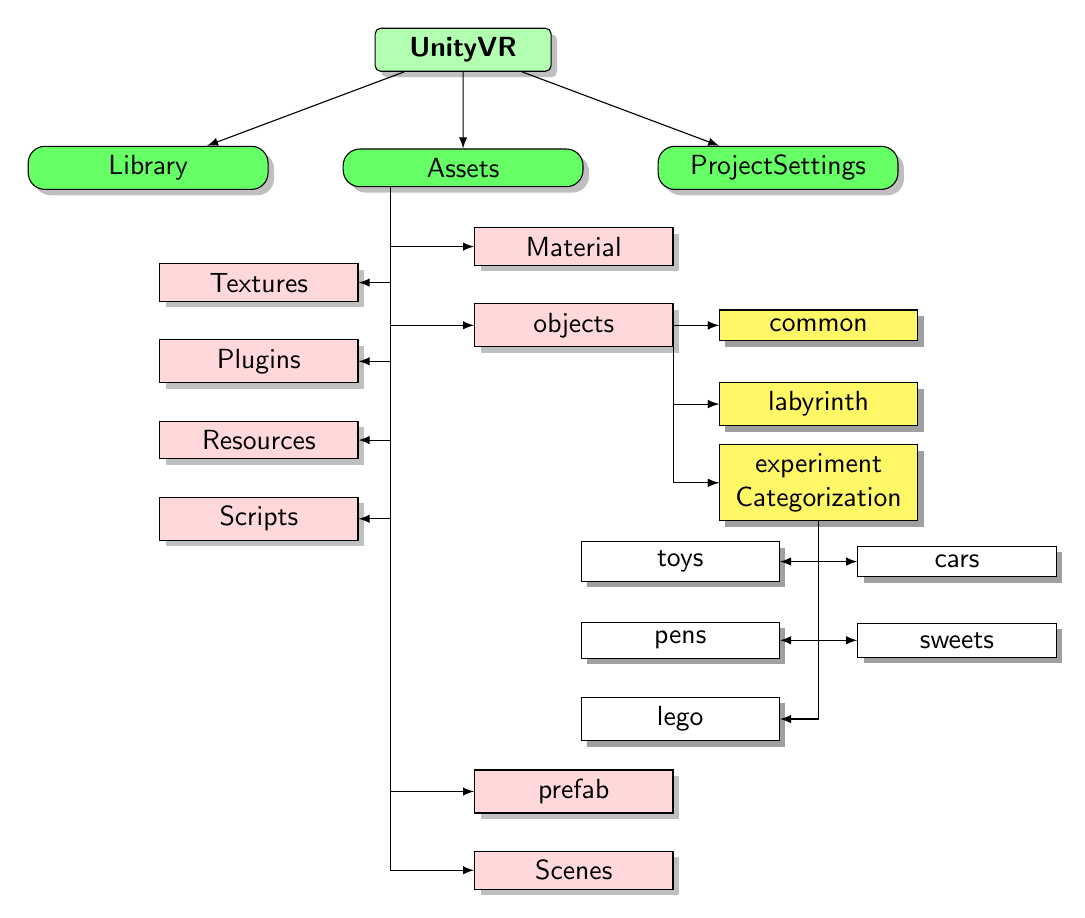
\begin{tikzpicture}[
  level 1/.style={sibling distance=40mm},
  edge from parent/.style={->,draw},
  >=latex]

% root of the the initial tree, level 1
\node[root] {\textbf{UnityVR}\\ }
% The first level, as children of the initial tree
  child {node[level 2] (c2) {Library}}
  child {node[level 2] (c1) {Assets}}
  child {node[level 2] (c3) {ProjectSettings}};  

% The second level, relatively positioned nodes
\begin{scope}[every node/.style={level 3}]
\node [below of = c1, xshift=40pt] (c11) {Material};
\node [below of = c11] (c12) {objects};
\node[level 4,right of = c12,xshift=60pt] (c110) {common};
\node[level 4,below of = c110] (c111) {labyrinth};
\node[level 4,below of = c111] (c112) {experiment\\Categorization};
\node[level 5,below of = c112,xshift=50pt] (c1120) {cars};
\node[level 5,below of = c112,xshift=-50pt] (c1121) {toys};
\node[level 5,below of = c1120] (c1122) {sweets};
\node[level 5,below of = c1121] (c1123) {pens};
\node[level 5,below of = c1123] (c1124) {lego};
\node [below of = c12,yshift=-140pt] (c13) {prefab};
\node [below of = c13] (c14) {Scenes};
\end{scope}

\begin{scope}[every node/.style={level 3}]
\node [below of = c2, xshift=40pt,yshift=-13pt] (c21) {Textures};
\node [below of = c21] (c22) {Plugins};
\node [below of = c22] (c23) {Resources};
\node [below of = c23] (c24) {Scripts};
\end{scope}


% lines from each level 1 node to every one of its "children"
\foreach \value in {1,2,3,4}
  \draw[->] (c1.195) |- (c1\value.west);

\foreach \value in {1,2,3,4}
  \draw[->] (c1.195) |- (c2\value.east);


\foreach \value in {0,1,2}
  \draw[->] (c12.east) |- (c11\value.west);

\foreach \value in {0,1,2}
  \draw[->] (c12.east) |- (c11\value.west);

\foreach \value in {0,2}
  \draw[->] (c112.south) |- (c112\value.west);

\foreach \value in {1,3,4}
  \draw[->] (c112.south) |- (c112\value.east);




\end{tikzpicture}
\end{center}
\dirtree{%
.1 UnityVR\DTcomment{Main project folder}.
.2 Assets\DTcomment{This is the main folder of the Project View in the IDE}.
.3 Materials\DTcomment{Created by Unity for materials}.
.3 objects\DTcomment{Imported objects}.
.3 Plugins\DTcomment{Additional assemblies}.
.3 prefab\DTcomment{Prefabs (see chapter \ref{prefabs})}.
.3 Resources\DTcomment{Contains objects that are loaded at runtime via \emph{Resources.Load(...)}}.
.3 Scenes\DTcomment{Contains all scene files}.
.3 Scripts\DTcomment{Contains all scripts}.
.3 Textures\DTcomment{created by Unity for textures}.
.2 Library\DTcomment{Cache of Unity}.
.2 ProjectSettings\DTcomment{Various setting files created by Unity}.
}
\end{comment}

\begin{figure}[h]
\begin{center}
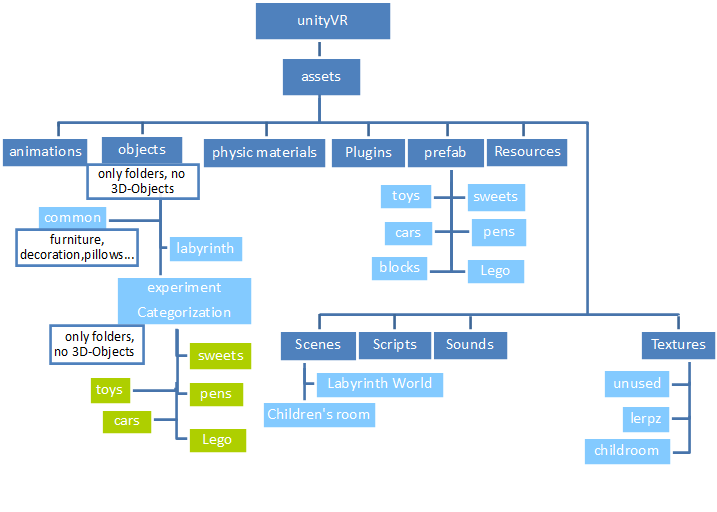
\includegraphics[width=0.9\textwidth]{images/ordnerstruktur.png}
\end{center}
\caption{Folder structur}
\label{folderstructure}
\end{figure}


\begin{tabular}{|l|l|}
\hline
Directory & Description\\\hline
Assets & This is the main folder of the Project View in the IDE\\
animations & Contains the agents and animations\\
objects & Contains all used objects\\
objects/common & Basic and environment objects\\
objects/labyrith & Specialized objects only used in the Labyrinth scene\\
objects/experiment categorization&  Specialized objects only used in the categorization experiment \\
physic materials & Demonstration of physic materials like rubber balls\\
Plugins & Additional .NET assemblies like SimpleNet.dll\\
prefab & Prefabs (see chapter \ref{prefabs})\\
Resources & Contains objects that are loaded at runtime via \emph{Resources.Load(...)}\\
Scenes & Contains all scene files\\
Scripts & Contains all scripts\\
Sound & Reserved for future usage\\
Textures & Created by Unity3D for textures\\\hline
\end{tabular}


%SECTION%%%%%%%%%%%%%%%%%%%%%%%%%%%%%%%%%%%%%%%%%%%%%%%%%%%%%%%%%%%%
\section{Classes}

Figure \ref{Classdiagram} shows the class diagramm of UnityVR. The two main classes of UnityVR are \emph{AgentScript} and \emph{BehaviorScript}. The \emph{AgentScript} is used to customize the behavior of an agent, while the \emph{BehaviorScript} is responsible for customizing the behavior of the environment.


\subsection{AgentScript}
\label{AgentScript}

\emph{AgentScript} is the main control script of an agent instance. It must be attached directly to the agent. This script is intended to be derived and the behavior of the agent can be modified by the virtual functions with \emph{"Process"} prefix which modify the processing of actions (see \ref{actions}). The following code shows all functions, which can be overridden, to create custom behavior.

\begin{lstlisting}
using System;
using System.Collections;
using SimpleNetwork;
using UnityEngine;

public class ExampleAgentScript : AgentScript
{
	protected virtual void ProcessMsgAgentGraspID(MsgAgentGraspID msg) { }

	protected virtual void ProcessMsgAgentGraspPos(MsgAgentGraspPos msg) { }

	protected virtual void ProcessMsgGraspRelease(MsgAgentGraspRelease msg) { }

	protected virtual void ProcessMsgAgentEyeFixation (MsgAgentEyeFixation msg) { }

	protected virtual void ProcessMsgAgentEyeMovement (MsgAgentEyemovement msg) { }
	
	protected virtual void ProcessMsgAgentPointID (MsgAgentPointID msg) { }

	protected virtual void ProcessMsgAgentPointPos (MsgAgentPointPos msg) { }

	protected virtual void ProcessMsgAgentTurn( MsgAgentTurn msg ) { }

	protected virtual void ProcessMsgAgentInteractionID (
		MsgAgentInteractionID msg) { }

	protected virtual void ProcessMsgAgentInteractionPos (
		MsgAgentInteractionPos msg) { }

	protected virtual void ProcessMsgAgentMovement (MsgAgentMovement msg) { }

	protected virtual void ProcessMsgAgentMoveTo(MsgAgentMoveTo msg) { }

	protected virtual void ProcessMsgAgentCancelMoveTo(MsgAgentCancelMoveTo msg) { }
	  
	protected virtual void ProcessMsgAnnarNetwork(AnnarNetwork msg) { }

	protected virtual void ProcessMsgAnnarUpdateRates(AnnarNetwork msg) { }
}
\end{lstlisting}
\subsection{BehaviorScript}

\emph{BehaviorScript} is the main control script for the environment. It stores all references to agent objects and all attached \emph{AgentScript}s from the scene. It also initializes the \emph{AgentScript}s. All agent objects must have the "agent" tag, otherwise \emph{BehaviorScript.AgentInitalization} can not find the agents automatically.
A minimal example of a \emph{BehaviorScript} which initializes the agents looks like this: 

\begin{lstlisting}
using System;
using System.Collections;
using SimpleNetwork;
using UnityEngine;
public class ExampleBehaviorScript : BehaviourScript
{
    protected override void AgentInitalization()
    {
        getAllAgentObjects<ExampleAgentScript>();
        getAndInitAllAgentScripts<ExampleAgentScript>();
    }
}
\end{lstlisting}


The following listing shows all possible functions which can be overridden. Mark that these functions are within the class.

\begin{lstlisting}

    protected virtual void ProcessMsgEnvironmentReset (MsgEnvironmentReset msg)
    {	
    	//custom EnvironmentReset behavior 		
    }

    protected virtual void ProcessMsgTrialReset (MsgTrialReset msg)
    {
      	//custom TrialReset behavior
    }

\end{lstlisting}


\begin{figure}[h]
\begin{center}
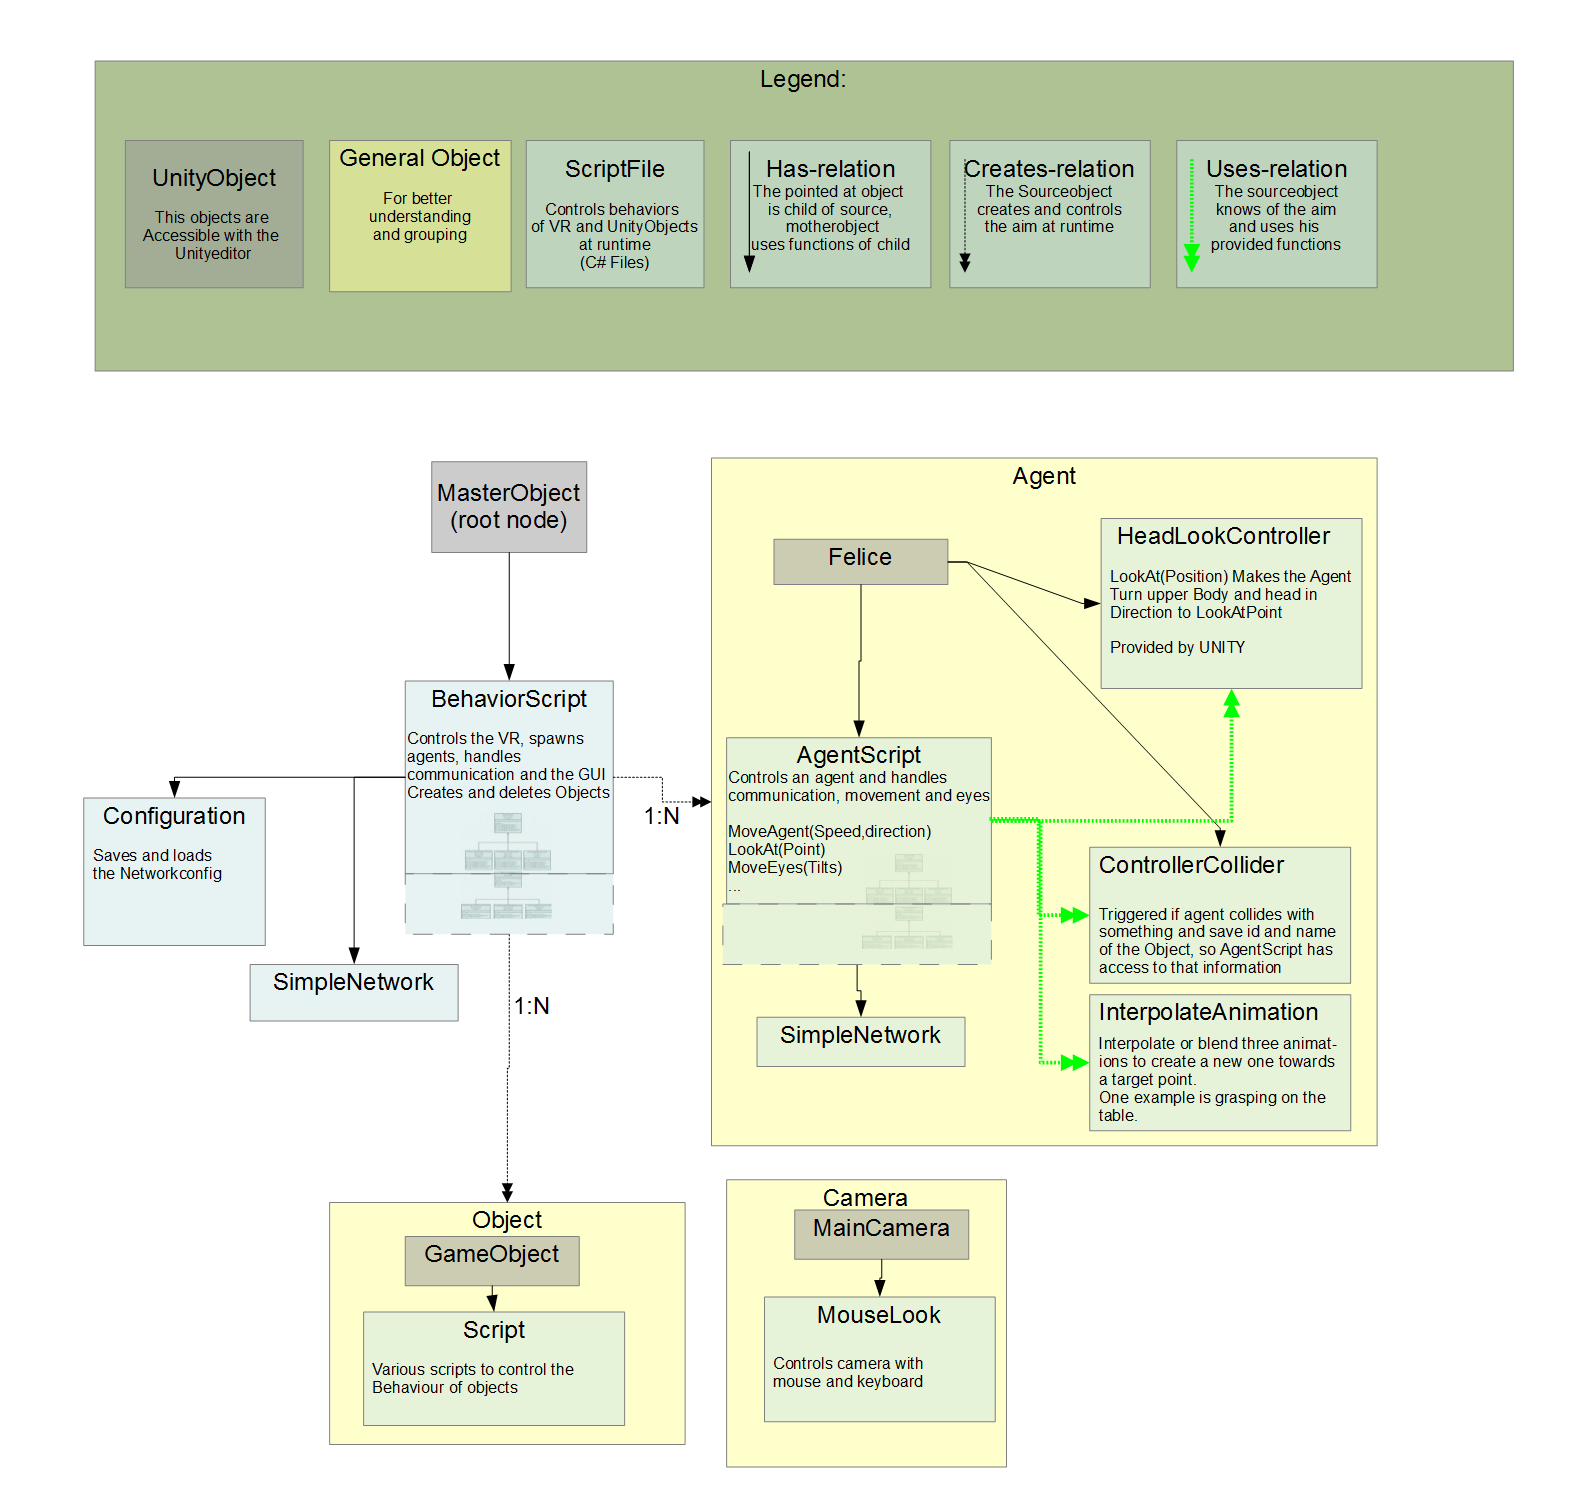
\includegraphics[width=0.9\textwidth]{images/VR-Classdiagram.png}
\end{center}
\caption{UnityVR Class diagram. AgentScript and BehaviourScript are intended to be derived, so that each agent and each environment has its own behavior.}
\label{Classdiagram}
\end{figure}

\newpage

\section{Agents}
At the moment (17. December 2015) there are two agents included in UnityVR, Lerpz and Felice. Lerpz was the first agent which was included and has only some limited animation capabilities. Felice has a full set of grasp animations. The feature to grasp an object (described in \ref{grasppos} and \ref{grapobj}) is only usable with Felice. 

\begin{figure}[h]
\begin{center}
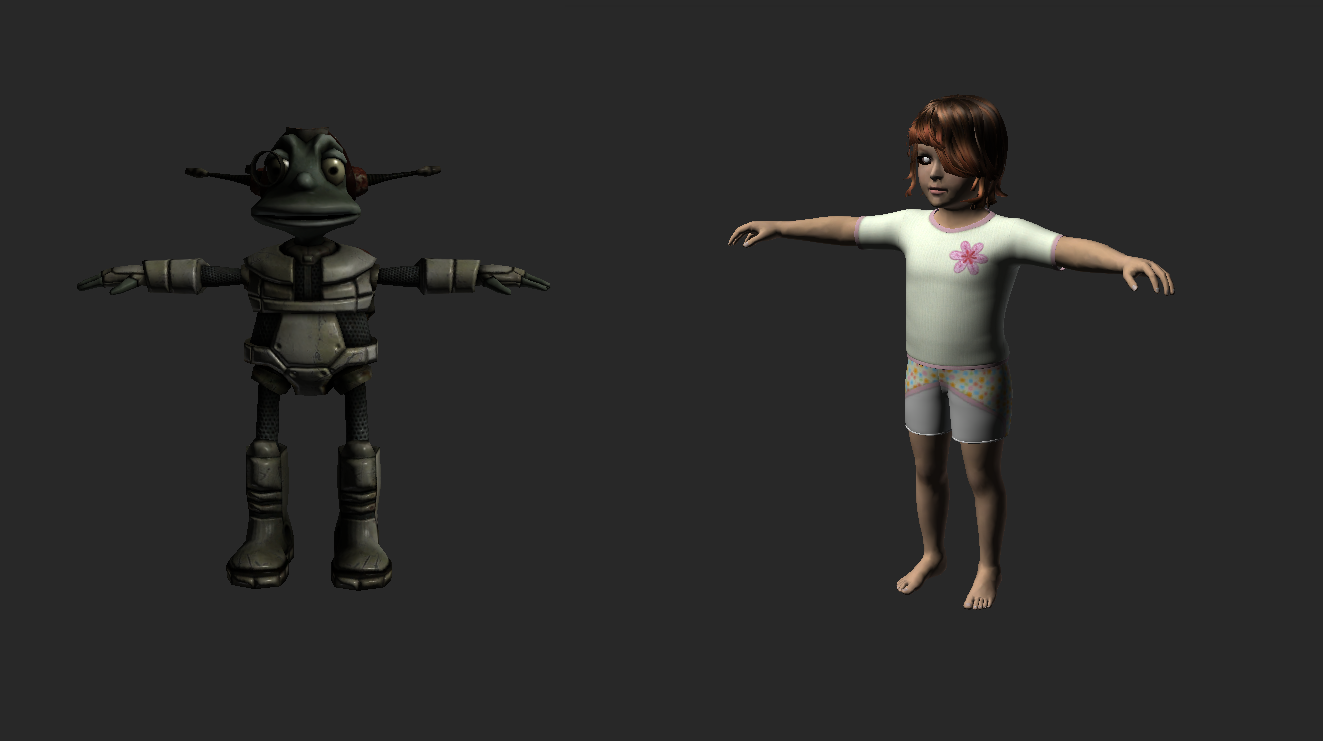
\includegraphics[width=0.95\textwidth]{images/agents.png}
\end{center}
\caption{ Lerpz (left) and Felice (right), the two agents which are included in UnityVR.}
\label{imgagents}
\end{figure}
\subsection{Sensors}
The agent has the following sensors similar to a human.
\begin{itemize}
\item Collision detection
\item Eye cameras
\item Agent position (intended for debugging)
\end{itemize}


\subsection{Actions}
\label{actions}
The agent can execute the following actions.
\begin{itemize}
\item Execute a movement of the agent
\item Rotation of the eyes
\item Fixation of the eyes
\item Grasping to a position with the right hand
\item Grasping to a certain object with the right hand
\item Point at an object with the right hand
\item Point to a position with the right hand
\item Interact with an object
\item Interact with a position
\end{itemize}



\section{Animations}
All informations  about using and creating animations are described in:
\begin{itemize}
\item unityVR/doc/animation-3Dobjects/daz/animationDocu
\end{itemize}


For a full overview of the animation capabilities of Unity3D refer to \url{http://docs.unity3d.com/Documentation/Manual/CreatingGameplay.html}. With Unity3D 4.0, a new animation system was introduced. Since the project started with
Unity3D 3.5, UnityVR uses the \emph{Legacy animation system}.


\section{Animate actions}

Animations are used to illustrate the execution of actions. They are necessary for grasping, pointing and interaction with objects. 

\subsection{Grasp to a Specific Position}
\label{grasppos}

\emph{Felice} is able to grasp to custom position. The following code shows an example where the \emph{GraspToPos} function can be used to grasp to a specific position in World Space coordinates.

\begin{lstlisting}
InterpolateAnimations interpolateAnimations;

void Start () 
{			
	interpolateAnimations = new InterpolateAnimations(this, "Assets/animations/feliceTarget.csv");	
	ArmAnimationList = ArmAnimationList.Union(interpolateAnimations.animationArray.ToList()).ToList();			
}

void GraspToPos(float x, float y, float z)
{
	interpolateAnimations.animate(x,y,z);
}
\end{lstlisting}

\subsection{Grab an Object}
\label{grapobj}

To get \emph{Felice} to grab an object with her right hand, you need to 

\begin{itemize}
\item Attach the \emph{HandCollider} script to the right hand of \emph{Felice}. You find the right hand via
Felice \(\rightarrow\) Genesis \(\rightarrow\) hip \(\rightarrow\) abdomen \(\rightarrow\) abdomen2 \(\rightarrow\) chest \(\rightarrow\) rCollar \(\rightarrow\) rShldr \(\rightarrow\) rForeArm \(\rightarrow\) rHand 
\item Attach a \emph{SphereCollider}
\begin{itemize}
\item Set \emph{Position} to [2,-1,1]
\item Set \emph{Radius} to 4
\item Turn \emph{IsTrigger} off
\end{itemize}
\item Attach a \emph{Rigidbody} to the right hand
\begin{itemize}
\item Turn on the \emph{Freeze Position} and \emph{Freeze Rotation} of all coordinates
\item Turn \emph{UseGravity} off
\end{itemize}
\item Change the tag of the right hand to "agentHand"
\item Attach a collider and Rigidbody on the target object
\item Change the tag of the object to "usable"
\end{itemize}
Now, when the right hand collides with an tagged object, the object is attached to the hand.

Releasing of an grasped object can be done by the following function:

\begin{lstlisting}
void ReleaseObject()
{
	if(rightGraspedObject != null)
	{
		//change parent to global one, this releases the object
		rightGraspedObject.transform.parent = null;
		rightGraspedObject.rigidbody.useGravity = true;   // enable gravity
		rightGraspedObject.rigidbody.isKinematic = false; // enable pyhsics
		//mark object as released
		rightGraspedObject = null;
	}
}
\end{lstlisting}

\section{Config file --- APPConfig.config}
\label{appconfig}

The \textsf{APPConfig.config} is located in the project root folder. 

\begin{lstlisting}
<?xml version="1.0" encoding="UTF-8"?>
<cConfiguration xmlns:xsi="http://www.w3.org/2001/XMLSchema-instance" xmlns:xsd="http://www.w3.org/2001/XMLSchema">
  <LocalPort>1337</LocalPort>
  <SyncMode>false</SyncMode>
  <SimulationTimePerFrame>0.1</SimulationTimePerFrame>
  <ImageResolutionWidth>1024</ImageResolutionWidth>
  <SendGridPosition>true</SendGridPosition>
  <MovementSpeed>3</MovementSpeed>
  <CameraDisplayWidth>512</CameraDisplayWidth>
  <FovHorizontal>120</FovHorizontal>
  <FovVertical>90</FovVertical>
</cConfiguration>
\end{lstlisting}


\begin{tabular}{|l|p{10cm}|}
\hline
Option & Description\\\hline\hline
LocalPort & The local port for the TCP connection for the ANNarchy client\\
SyncMode &  Switch between the synchronous/asynchronous mode (see \ref{SyncMode})\\
SimulationTimePerFrame & The simulation times in seconds. Precisely, the time between two send time points of the images. In synchron mode, the sending is always executed in the first frame, therefore it is the simulated time of 2 frames. In asychron mode, we wait at least "SimulationTimePerFrame" seconds.\\
ImageResolutionWidth & Width in pixel for the rendered eye camera images in the scene\\
ImageResolutionHight & (obsolet) Height in pixel for the rendered eye camera images in the scene\\
SendGridPosition & If turned on, the Agent sends its position data in every frame to the Client.\\
MovementSpeed & Movement speed of the agent\\
CameraDisplayRes & Width \& Height of the rendered eye images which will be sent to the client.\\
FovHorizontal & Field of View in degree of the horizontal\\
FovVertical & Field of View in degree of the vertical \\\hline
\end{tabular}

\section{Synchron Mode}
\label{SyncMode}

For a full overview refer \emph{unityVR/doc/VR-doc/synchronDescription.pdf}.

The UnityVR could operate in two modes: synchronous and asynchronous. This can be changed in the
configuration file with the \emph{SyncMode} parameter (synchronous mode = true).\\
The purpose of the synchronous mode is that the agent and the VR use the same time scales. To ensure this,
the simulation time scale is independent from the calculation time of the agent and the VR. Such equal time
scales are essential to simulate a scientific experiment. The simulation time is sliced into periods and the VR and agent are synchronized at the end of each periode.\\
The synchronization occurs in the following order. First, the agent receives its input and a \emph{MsgStartSync}
message indicating that the agent simulation could start. Then, the agent has enough calculation time to process
input information as the VR is paused until the agent has processed all data and has sent all motor commands
back. This is indicated by an \emph{MsgStopSync} message sent by the agent to the VR.
The synchronization protocol is split over two frames of the VR.

\begin{itemize}
\item In the first frame, the VR sends the \emph{MsgStartSync} message and all sensor data, like images and location,
to the agent. The VR continues to the second frame. Now the agent should process the data and send
motor actions back to the VR. The last messages, which the agent must send back, is \emph{MsgStopSync}.
\item The VR remains in the second frame and processes all motor messages from the agent until it received
the \emph{MsgStopSync}.
\end{itemize}

The time scale is controlled by the value of \emph{SimulationTimePerFrame} which can be changed in the configuration
file. It determines the interval of sending images. In asynchronous mode, it is the interval in real time, hence the
images are sent after this time period has passed. In synchronous mode, \emph{SimulationTimePerFrame} determines
the simulation time period. As the images are sent always in Frame 1, it is how much time is simulated over 2
frames in an experiment.
For the case that the \emph{MsgStopSync} is lost, there is a timeout implemented in the second frame.


\section{Connection with ANNarchy}
\label{ConnectionwithANNarchy}

UnityVR can be connected to the ANNarchy library via network (tcp/ip and protobuf). To do so, you must install the following tools: 	

\begin{enumerate}
\item If you want to develop/modify the virtual reality, we advise you to use Visual Studio 2010. A development project of the virtual reality could be started via unityVR/unityVR\_xxx/unityVR\_xxx.sln. If it does not exist, it will be generated by opening a script/asset in Unity. The main project description can be found under unityVR/doc/VR-doc/html/index.html .
%\item Build the SimpleNetwork project which is placed under unityVR/SimpleNetwork . Do not debug or run it. 
\item  Protobuf-C++ library (\url{http://code.google.com/apis/protocolbuffers/docs/overview.html}) is a fast and lightweight serializer, intended to use for network transfer. It can normally be found in the repositories of your linux distribution. For ubuntu 10.04, the necessary packages are libprotobuf-dev and protobuf-compiler. Do NOT install  protobuf-c-compiler or libprotobuf-c0-dev, these are pure c version. To avoid troubles, install protobuf-2.5.0.
\item If you choose ANNarchy 4: Consult \emph{agentBrain/networkAnnarchy4/python/readme.txt} in addition. Currently, the following steps should allow you to connect and execute e.g. \newline \emph{agentBrain/networkAnnarchy4/python/test\_cases.py}
\begin{enumerate}
\item Execute \emph{agentBrain/networkAnnarchy4/recompileProtoc.sh} .
\item Import the project in the \emph{agentBrain/networkAnnarchy4/} directory into Eclipse and build it.
\item Copy \emph{agentBrain/networkAnnarchy4/Debug/libann4VrInterfaceCpp.so} to \emph{agentBrain/networkAnnarchy4/libs/} .
\item Enter the IP address to the VR at the end of \textsf{test\_cases.py} and run this file via python command while the VR is running.
\end{enumerate}
\item If you choose ANNarchy 2.3: 
\begin{enumerate}
\item Compile your ANNarchy 2.3 application with network support. For this, execute \textsf{recompileProtoc.sh} and afterwards you must simply add PROTOC=1 after the scons command (see above), eg. \textsf{> scons  GUI=0 DEBUG=1 PROTOC = 1}  OR call the installscript with - -protoc: \textsf{> python script/installANNarchy.py - -protoc} .
\item An example could be found in: \emph{agentBrain/networkInterfaceCPP/Tests}. For this, you should use eclipse+cdt as IDE, since the directory contains an eclipse-project file (.project). You can start the example by first starting the unity-project, then click at run (the arrow) and finally compile \& start the agent (c++ project).
\end{enumerate}
\end{enumerate}


\chapter{Further Information}

This chapter covers some more infomation and tips about working with Unity3D, the UnityVR and 3D objects.

\section{Duplicate an Object of the Project}

In the  context menu of an item in the Unity3D Project View, there is no option to duplicate it. The hidden function to do this, is to select the item and press Strg-D.


\section{Prefabs}
\label{prefabs}

Prefabs are types of assets. They are used to create a reusable \emph{GameObject} which can be used in other scenes and to create instances at runtime. If you change properties in a prefab, it is automatically applied to all instances of that prefab.

\subsection{Creating a Prefab}

\begin{enumerate}
\item Create your desired object in the scene editor. Attach all components and scripts.
\item Create an empty prefab in the Project View (right click) and drag the object from the Scene View onto the empty prefab in the Project View.
\end{enumerate}

\subsection{Instantinate Prefabs at Runtime}

The prefab must be located in the \emph{Resources} folder, otherwise Unity3D can not find it at runtime.

As an example, the following code loads the \emph{Lerpz} agent into the scene which is located as a prefab in the \emph{Resources} folder:

\begin{lstlisting}
Instantiate(Resources.Load("Lerpz") as UnityEngine.Object, new Vector3( 0 , 0, 0), Quaternion.identity);
\end{lstlisting}



For more information about the \emph{Instantiate} function look at \url{http://docs.unity3d.com/Documentation/ScriptReference/Object.Instantiate.html}


\section{Multiple Agents}

In UnityVR it is also possible to put more than one agent into the scene. Each agent has its own TCP socket to communicate with its client. There are two ways to achieve this.

\begin{enumerate}
\item The first method is to create all the agents inside the Unity3D editor (like in \ref{createagent}) and change the \emph{AgentID} of all attached \emph{AgentScript}s to ascending integers (0, 1, 2, 3, etc.).
\item The second method is used in the Labyrith scene. It is also an example of using prefabs. Lerpz (the agent) is stored as a prefab in the \emph{Assets/Resources}. It is than instantinated
at runtime. The following code is taken from \emph{Asserts/Scripts/LabyrithBehaviorScript.cs}. It spawns three instances of Lerpz at runtime.
\end{enumerate}
\begin{lstlisting}
protected override void AgentInitalization()
{
	const int numberOfAgents = 3;	
	agents = new GameObject[numberOfAgents];

	for(int i = 0; i < numberOfAgents; i++)
	{
		//Position for agent x_i = (0,-20,20,-40,40,-60,60,....)	
		float pos = Mathf.Pow( -1,i ) * 20 * Mathf.Ceil(i/2f);
			
		agents[i] = Instantiate(Resources.Load("Lerpz") as UnityEngine.Object, new Vector3( pos , 0, 0), Quaternion.identity) as GameObject;

		agents[i].GetComponent<LabyrinthAgentScript>().AgentID = i;            	
							
		//Get the Agent ready
		agents[i].GetComponent<LabyrinthAgentScript>().DefaultAgentPosition = new Vector3( pos , 0, 0);			
	}	
		
		
	// find and init all agent SCRIPTS  in the scene containing a specific script
	getAndInitAllAgentScripts<LabyrinthAgentScript>();
		
	//prevent that several cameras are rendered at top of each other: allow only first agent to display camera		
	for(int i = 1; i < numberOfAgents; i++)
		agentScripts[i].setDisplayCameraVR(false);
		
}
\end{lstlisting}


\section{Working with 3D Objects}
\subsection{3D Libary}

In this library you will find objects which are not included in our UnityVR project.
Our 3D library includes many Objects in different categories:

\begin{enumerate}
\item Accessories (common, pillows, veils, ...)
\item Blocks (Lego, cubes)
\item Cars
\item ChildVersion1 (this is our first version of the child felice)
\item Felice (the first animations of felice)
\item Neuron
\item Pens
\item Sweets
\item Toys
\end{enumerate}

The pictures (.jpg) show you the preview of the objects. So you do not have to open every object. The files have the extensions .3DS, .blend and .fbx.\\
The .fbx format is the best format for exporting and importing objects. This format is the only one which supports the import of animations into Unity3D. For example, the maya (and 3DS) format do not support animations. Additionally, these formats should not even be used for simple 3D objects as they require the maya software for opening these objects.

\subsection{Textures in Max 3D}
In Max 3D you can change or rename the materials and textures of your objects. Also, you can increase or decrease them. 
The following three links will show how to work with textures and materials in Max 3D and how to export them.

\begin{itemize}
\item \url{http://www.youtube.com/watch?v=zLMv1KUy8ZQ}
\item \url{http://www.youtube.com/watch?v=5lSANYBzQAI}
\item \url{http://www.youtube.com/watch?v=VNaXrWcbQfw} 
\end{itemize}

\end{document}
